% RA-L initial submissions use the RAS conference layout.
\documentclass[letterpaper,10pt,conference]{ieeeconf}
\IEEEoverridecommandlockouts
\overrideIEEEmargins
\usepackage[T1]{fontenc}
\usepackage{times}
\usepackage{amsmath,amssymb,bm}
\usepackage{graphicx}
\usepackage{tikz}
\usetikzlibrary{arrows.meta}
\usepackage{cite}
\usepackage{balance}
\usepackage[hidelinks]{hyperref}
\newcommand{\vect}[1]{\bm{#1}}
\newcommand{\axis}{\hat{\vect z}_t}
\newcommand{\clip}{\operatorname{clip}}
\newcommand{\sgn}{\operatorname{sgn}}
\title{Learning Iterative Dynamic Regrasping with Limited Gripper Control}
% Replace according to the target submission's anonymity requirements.
\author{Author names and affiliations to be added}
\begin{document}
\maketitle
\thispagestyle{empty}
\pagestyle{empty}

\begin{abstract}
Dynamic regrasping allows a parallel gripper to reposition an object by coordinating arm motion with brief release and recapture. The achieved displacement depends on friction, arm tracking, and the effective release interval, making a predefined motion sensitive to execution errors. We formulate iterative axial regrasping as a partially observable control problem and train feedforward and recurrent policies using proximal policy optimization. The policy coordinates motion along a tilted grasp axis with gripper pulse requests and uses feedback to correct the remaining position error over successive attempts. A reduced contact model explains the competing effects of gravity, inertia, and lower-finger friction. Training in Genesis incorporates filtered arm commands, a constrained pulse mechanism, and randomized contact parameters. A gated recurrent unit retains observation history to address hidden actuator and contact states. OptiTrack provides object position measurements for the planned hardware evaluation. This manuscript presents the physical formulation and learning methodology; experimental validation remains to be completed.
\end{abstract}

\noindent\textbf{Index Terms---}Dexterous manipulation, reinforcement learning, manipulation planning.

\section{Introduction}
A grasp suitable for transporting an object may be poorly located for tool use or assembly. Repositioning the object within a parallel gripper can avoid placing it down and acquiring a new grasp. Although finger motion offers limited dexterity, arm acceleration and controlled release can generate relative object motion. The central challenge is to coordinate that motion with recapture and correct the remaining error without losing the object.

Extrinsic dexterity exploits gravity, external contacts, and arm dynamics to extend the capabilities of simple grippers~\cite{dafle2014extrinsic}. Shi et al.~\cite{shi2017sliding} developed a contact-based planner for inertial sliding and iterated execution to reduce modeling and tracking errors. Thus, iterative correction is already an established regrasping principle. Learning offers another means of selecting these actions: Wei et al.~\cite{wei2023regrasp} learned gravity-driven sliding from demonstrations, while Ma and Adelson~\cite{ma2025dynamic} combined planning, computed torque control, and asynchronous visual feedback for throwing and catching. These approaches motivate studying feedback during dynamic manipulation rather than treating a commanded trajectory as its exact physical execution.

The present task couples axial arm motion to brief gripper pulses. Opening requests do not uniquely determine release time: finger motion, residual squeeze, and friction affect when the object moves. Arm filtering and tracking likewise alter the velocity at release. At a tilted grasp, the released object may remain supported by the lower finger, making purely ballistic predictions inaccurate. A policy must therefore coordinate motion and contact transitions while using subsequent observations to correct each attempt.

We train multilayer perceptron (MLP) and gated recurrent unit (GRU) policies with proximal policy optimization (PPO)~\cite{schulman2017ppo}. Dynamics randomization motivates exposing the policies to contact variability~\cite{peng2018dynamics,openai2020dexterous}, while recurrence provides a mechanism for using history when relevant state is unobserved~\cite{ni2022recurrent}. Our focus is the combination of a constrained pulse interface, realized arm dynamics, and repeated axial error correction. The physical formulation below motivates this design; the methodology specifies its implementation and the intended OptiTrack feedback interface. Neither an advantage of GRU over MLP nor successful hardware transfer is assumed.

\section{System and Physical Formulation}
\label{sec:physics}
\begin{figure}[t]
 \centering
 % Adapted from reports/regrasp_pulse_math/fbd_section.tex.
% Editable vector artwork; compact labels for a single-column manuscript.
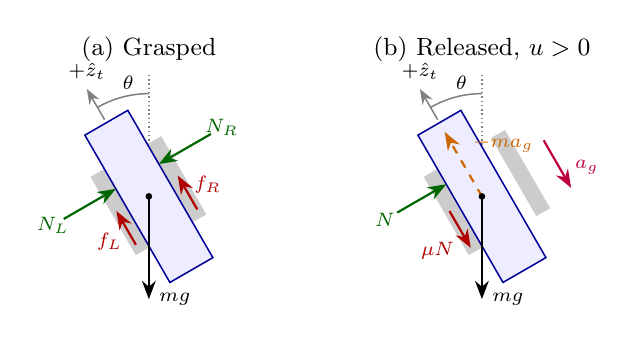
\begin{tikzpicture}[x=0.45cm,y=0.45cm,>=Stealth,
  every node/.style={font=\scriptsize},line width=0.55pt]
  \begin{scope}
    \node[font=\small] at (0,4.15) {(a) Grasped};
    \draw[densely dotted,gray] (0,0) -- (0,3.5);
    \begin{scope}[rotate=30]
      \fill[gray!40] (-1.15,-1.25) rectangle (-0.7,1.3);
      \fill[gray!40] (0.7,-1.25) rectangle (1.15,1.3);
      \filldraw[fill=blue!7,draw=blue!60!black] (-0.7,-2.4) rectangle (0.7,2.4);
      \draw[->,gray] (0,2.5) -- (0,3.5) node[above,text=black] {$+\hat z_t$};
      \draw[->,thick,green!40!black] (-2.4,0.65) -- (-0.7,0.65);
      \node[green!40!black] at (-2.75,0.65) {$N_L$};
      \draw[->,thick,green!40!black] (2.4,0.65) -- (0.7,0.65);
      \node[green!40!black] at (2.75,0.65) {$N_R$};
      \draw[->,thick,red!70!black] (-1,-1) -- (-1,0.1);
      \node[red!70!black] at (-1.6,-0.55) {$f_L$};
      \draw[->,thick,red!70!black] (1,-1) -- (1,0.1);
      \node[red!70!black] at (1.6,-0.55) {$f_R$};
    \end{scope}
    \fill (0,0) circle (1.2pt);
    \draw[->,thick] (0,0) -- (0,-2.9) node[right] {$mg$};
    \draw[gray] (0,2.9) arc (90:120:2.9);
    \node at (-0.58,3.2) {$\theta$};
  \end{scope}
  \begin{scope}[shift={(9.4,0)}]
    \node[font=\small] at (0,4.15) {(b) Released, $u>0$};
    \draw[densely dotted,gray] (0,0) -- (0,3.5);
    \begin{scope}[rotate=30]
      \fill[gray!40] (-1.15,-1.25) rectangle (-0.7,1.3);
      \fill[gray!40] (1.05,-1.25) rectangle (1.5,1.3);
      \filldraw[fill=blue!7,draw=blue!60!black] (-0.7,-2.4) rectangle (0.7,2.4);
      \draw[->,gray] (0,2.5) -- (0,3.5) node[above,text=black] {$+\hat z_t$};
      \draw[->,thick,green!40!black] (-2.3,0.8) -- (-0.7,0.8);
      \node[green!40!black] at (-2.7,0.8) {$N$};
      \draw[->,thick,red!70!black] (-1,0.1) -- (-1,-1.1);
      \node[red!70!black] at (-1.85,-0.7) {$\mu N$};
      \draw[->,thick,dashed,orange!80!black] (0,0) -- (0,2.1);
      \node[orange!80!black,anchor=west] at (0.28,1.55) {$-ma_g$};
      \draw[->,thick,purple] (2.3,0.5) -- (2.3,-1.05);
      \node[purple,anchor=west] at (2.45,-0.45) {$a_g$};
    \end{scope}
    \fill (0,0) circle (1.2pt);
    \draw[->,thick] (0,0) -- (0,-2.9) node[right] {$mg$};
    \draw[gray] (0,2.9) arc (90:120:2.9);
    \node at (-0.58,3.2) {$\theta$};
  \end{scope}
\end{tikzpicture}

 \caption{Parallel-gripper regrasping, adapted from the project's pulse analysis. (a) Before release, opposing normals $N_L,N_R$ and tangential forces $f_L,f_R$ hold the bar. (b) During upward relative slip, the lower finger supplies normal $N$ and opposing friction $\mu N$. Gravity acts vertically; $-ma_g$ is the inertial force in the accelerating gripper frame. The upper-finger gap is exaggerated.}
 \label{fig:gripper}
\end{figure}

\subsection{Task and Coordinates}
A Franka arm holds a simulated $35$~g bar measuring $25\times25\times150$~mm. Fig.~\ref{fig:gripper} shows the grasp and release configurations. A fixed task frame $Q_t=[\hat{\vect x}_t\ \hat{\vect y}_t\ \axis]$ is defined at home, with grasp axis $\axis$ tilted by $\theta\in[0,45^\circ]$ from vertical. For object center $\vect p_o$ and fingertip midpoint $\vect p_f$, define
\begin{equation}
 \vect r=Q_t^\top(\vect p_o-\vect p_f),\qquad e=r_z-r_z^\star.
 \label{eq:relative}
\end{equation}
The goal is to reduce $|e|$ and finish in a settled grasp. Positive targets are sampled uniformly from $[12.5,22.5]$~mm with initial $r_z\simeq0$; negative and mixed-sign targets are also supported. Inclination is fixed for a training run and is not observed by the policy. Hand position $z_h$ is its displacement along $\axis$ from home plus a fixed offset $z_0=0.8546$~m; at nonzero tilt it is not world height.

\subsection{Release Dynamics and Timing}
Let $t_r,t_c$ be effective release and recapture times and $T=t_c-t_r$. Define $s(t)=r_z(t_r+t)-r_z(t_r)$ and relative velocity $u=\dot s$. Assuming axial gripper acceleration $a_g$, negligible object rotation, and contact with the lower finger in Fig.~\ref{fig:gripper}(b), the transverse gravity load gives $N\simeq mg\sin\theta$, where $m$ is object mass and $g$ is gravitational acceleration. With Coulomb coefficient $\mu$,
\begin{equation}
 \ddot s=-a_g-g\cos\theta-\mu g\sin\theta\,\sgn(u).
 \label{eq:dynamics}
\end{equation}
At $u=0$, sticking is possible when $|-a_g-g\cos\theta|\leq\mu g\sin\theta$. Consequently, maximum downward acceleration $A$ initiates upward slip from rest only if $A>g(\cos\theta+\mu\sin\theta)$. Tilting reduces axial gravity but increases friction opposing upward slip. The model neglects compliance, residual squeeze, and rotation; its friction term vanishes if lower-finger contact is lost.

For an ideal velocity reversal from $+V$ to $-V$ at acceleration $-A$, reversal requires $2V/A$. With the reference limits $V=0.45$~m/s and $A=15$~m/s$^2$, this is $60$~ms. The useful displacement, however, depends on the realized motion throughout release:
\begin{equation}
 s(T)=\int_{t_r}^{t_c}(v_o-v_g)\,dt,\qquad
 \frac{\partial s}{\partial T}=u(T),
 \label{eq:slip}
\end{equation}
where $v_o,v_g$ are axial object and fingertip-midpoint velocities and the derivative holds for fixed release and motion history. Closing after the relative-motion apex loses displacement when $u(T)<0$. Reference limits do not bound the realized motion under tracking overshoot, and commanded opening duration is not the effective release interval. These dependencies motivate learning pulse coordination and using feedback across repeated attempts.

\section{Learning Methodology}
\subsection{Observation and Execution}
The task is partially observable because pulse phase, lockout timers, filter state, and contact parameters affect transitions but are hidden from the actor. The $50$~Hz observation is
\begin{equation}
 o_k=[z_h,\dot z_h,v_k^{\rm ref},\alpha_k^{\rm ref},F_l,F_r,
 r_z,r_x,r_y,r_z^\star]^\top,
\end{equation}
where $v_k^{\rm ref},\alpha_k^{\rm ref}$ are reference velocity and acceleration, and $F_l,F_r$ are simulated finger-contact-force magnitudes. Fixed scales normalize the channels. The three policy outputs are clipped to $[-1,1]$: one requests axial velocity and two request finger positions. With $\Delta=20$~ms,
\begin{equation}
 v_{k+1}^{\rm ref}=\clip(Va_{k,0},v_k^{\rm ref}-A\Delta,v_k^{\rm ref}+A\Delta).
\end{equation}
Position is integrated by the trapezoid rule and interpolated at $1$~kHz. A second-order velocity filter with natural frequency $75$~rad/s and damping ratio $0.33$ represents noninstantaneous arm response. A Cartesian controller holds orientation and transverse position while a damped Jacobian inverse maps the axial motion to joint velocities.

A rising threshold crossing of the mean finger request triggers a pulse. Pulses are blocked during the first $1$~s and for $1.2$~s after each accepted trigger. The pulse applies the policy's finger commands for $40$~ms, forces opening for $120$~ms, then commands closure for one $20$~ms step. Outside a pulse the fingers are commanded closed. The initial phase is therefore policy pass-through, not a guaranteed closed-gripper delay. Contact evolution determines the actual release and recapture times.

\subsection{Objective and Training}
With $\bar F=(F_l+F_r)/2$, release is detected at $\bar F<0.15$~N and the subsequent regrasp at $\bar F\geq0.75$~N. Event improvement is $\delta=|e^{\rm release}|-|e^{\rm regrasp}|$. The reward combines a terminal success bonus, bounded proximity shaping, regrasp improvement, and motion costs. The event term uses a capped quartic improvement bonus, penalizes worsening five times more strongly, and is paid only for the first four regrasps. Acceleration and acceleration-change costs suppress oscillation; an accepted pulse refunds the preceding six charged steps and exempts the trigger plus eight following steps, allowing purposeful acceleration. Speed and idle-motion costs discourage movement while waiting.

Success requires $|e|\leq5$~mm, $|\dot z_h|<0.05$~m/s, a firm grasp for at least three steps, and $z_h\in[0.70,0.86]$~m, with the conjunction held for five steps. Workspace violations, object escape, excessive finger closure, or a seventh regrasp terminate as failures; episodes time out after $9$~s. Thus passing through the desired position without settling is insufficient.

Both actor and critic use MLP layers of widths $(256,128,64)$ with ELU activations. The recurrent variant places a separate single-layer, $256$-unit GRU before each head, with actor state $h_k=\operatorname{GRU}(o_k,h_{k-1})$. State resets at episode boundaries. Both actors use Gaussian action distributions. PPO optimizes its clipped surrogate with generalized advantage estimates~\cite{schulman2016gae}, using $\gamma=0.99$, $\lambda=0.95$, clip $0.2$, initial learning rate $3\times10^{-4}$, target KL $0.01$, and five epochs over four minibatches. The value and entropy coefficients are $1$ and $0.005$. Existing MLP and GRU rollout lengths are $32$ and $64$ steps; this difference must be controlled in an architecture comparison. Recurrence may retain pulse history but is not explicitly trained to identify friction or delay.

Each reset samples friction from $\mathcal U[0.6,0.9]$ and finger stiffness from $\mathcal U[100,500]$~N/m. Optional observation noise is uniform within $\pm1$~mm for measured positions and $\pm1$~mm/s for hand velocity. Nominal pulse timing and filter parameters remain fixed: the current setup randomizes contact properties, not command latency.

\subsection{Planned Hardware Position Feedback}
OptiTrack supplies object pose in its measurement frame. The tracked marker pose must be transformed into the robot base frame and corrected for the marker-to-object-center offset; robot kinematics supply the fingertip midpoint. Time-aligned positions then enter (\ref{eq:relative}) using the same fixed task frame. Effective release timing and arm tracking must be characterized independently of pose-measurement latency. OptiTrack does not supply the two finger-force channels, so direct deployment additionally requires compatible contact sensing or a validated observation redesign. The available hardware workflow uses a Robotiq gripper, whose response cannot be assumed identical to the simulated Franka hand. Hardware validation and policy comparisons remain open experimental tasks.

% Add Experiments, Results, Discussion, and Conclusion after validation.
\balance
\bibliographystyle{IEEEtran}
\bibliography{references}
\end{document}
